\documentclass{beamer}
\usepackage[utf8]{inputenc}

\usetheme{Madrid}
\usecolortheme{default}
\usepackage{multicol}
\usepackage[]{algorithm2e}
\usepackage{amsmath, amssymb, amsfonts}
\usepackage{algorithm}
\usepackage{algpseudocode}
\usepackage{algcompatible}

\DeclareMathOperator*{\argmax}{argmax}  % in your preamble
\DeclareMathOperator*{\argmin}{argmin}  % in your preamble
\DeclareMathOperator{\EX}{\mathbb{E}}% expected value

%------------------------------------------------------------
%This block of code defines the information to appear in the
%Title page
\title[Off-Policy Algorithms] %optional
{Off-Policy Algorithms for Continuous Control (DDPG/TD3/SAC)}

\author[Khoa, Luc, Vu] % (optional)
{Khoa.~Tran\inst{1} \and Luc.~Truong\inst{2} \and Vu.~Huynh\inst{3}}

\\


\institute[] % (optional)
{
  \inst{1}%
  20520222
 `~
  \inst{2}%
  20520241 
  ~
  \inst{3}%
  20520864
  \\ \vspace{1.5cm}
    \large Class : CS106.M21.KHTN
    \\ \vspace{0.5cm}
    Supervisor: Dr. Luong Ngoc Hoang
}

\date[CS106] % (optional)
{July 08, 2022}

\logo{\includegraphics[height=1cm]{overleaf-logo}}

%End of title page configuration block
%------------------------------------------------------------



%------------------------------------------------------------
%The next block of commands puts the table of contents at the 
%beginning of each section and highlights the current section:

\AtBeginSection[]
{
  \begin{frame}
    \frametitle{Table of Contents}
    \tableofcontents[currentsection]
  \end{frame}
}
%------------------------------------------------------------


\begin{document}

%The next statement creates the title page.
\frame{\titlepage}


%---------------------------------------------------------
%This block of code is for the table of contents after
%the title page
\begin{frame}
        \frametitle{Table of Contents}
        \tableofcontents[2]
\end{frame}
%---------------------------------------------------------


\section{Continuous Control Problem}

%---------------------------------------------------------
%Changing visivility of the text
\begin{frame}
\frametitle{Continuous Control Problem}
    \begin{center}
        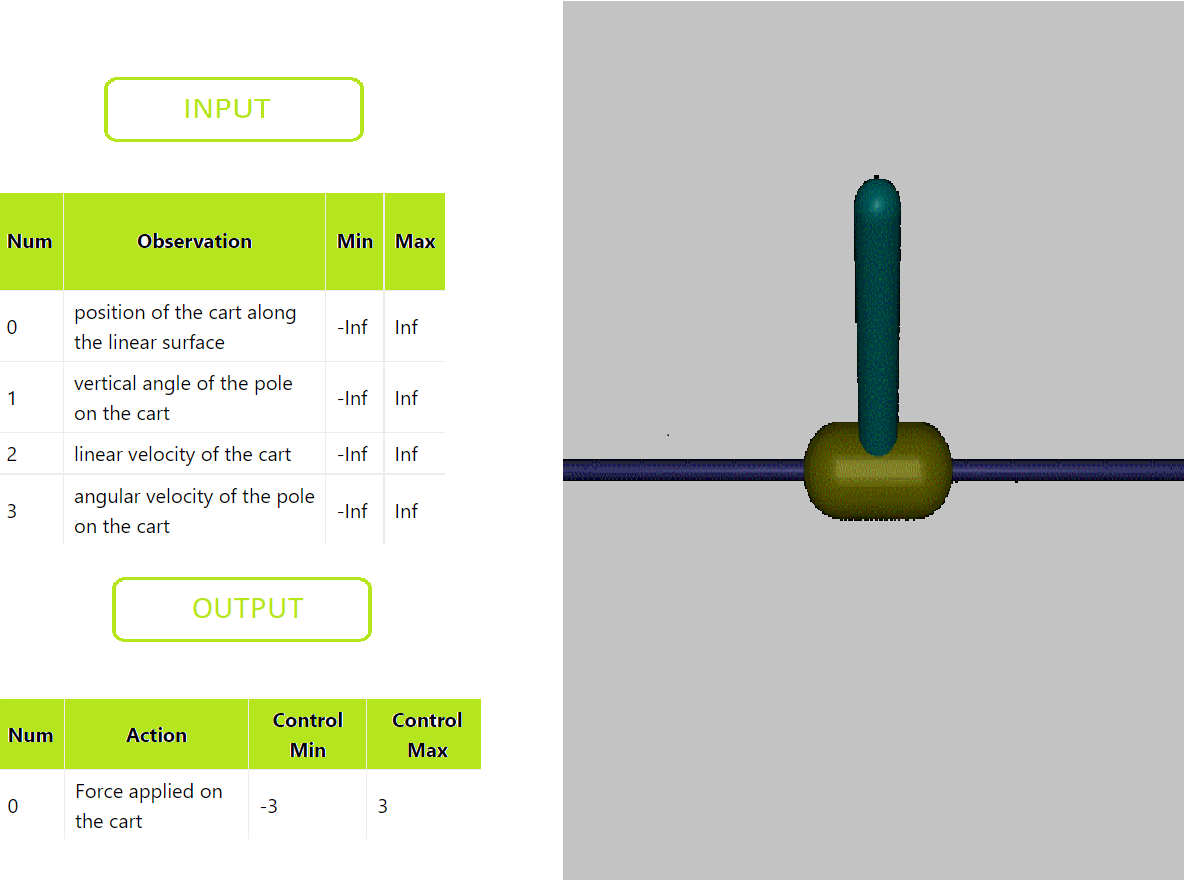
\includegraphics[scale=0.4]{problem1.png}
    \end{center}
\end{frame}

\begin{frame}
\frametitle{Continuous Control Problem}
    \begin{center}
        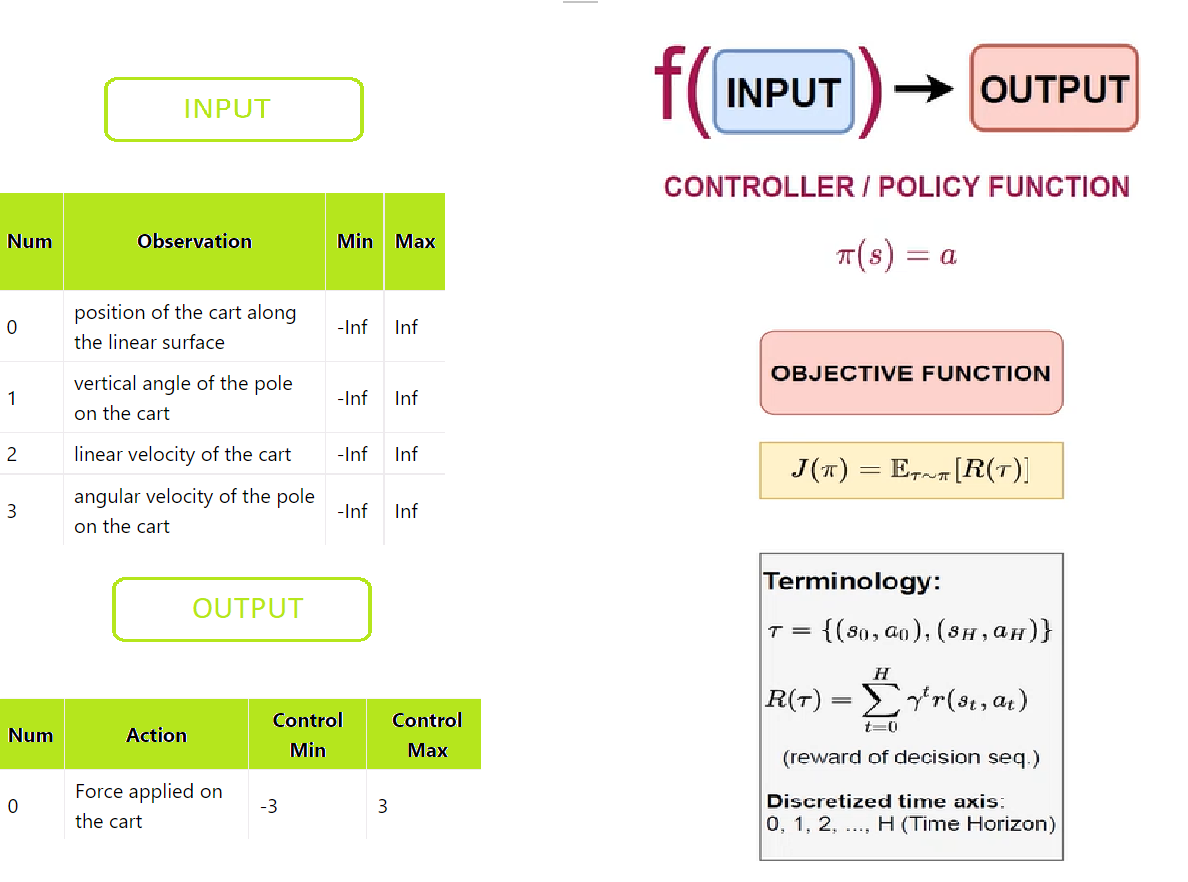
\includegraphics[scale=0.4]{problem2.png}
    \end{center}
\end{frame}

%---------------------------------------------------------

\section{Background}

\subsection{MDP and Reinforcement Learning (RL)}

\begin{frame}
\frametitle{MDP and Reinforcement Learning (RL)}
    \begin{center}
        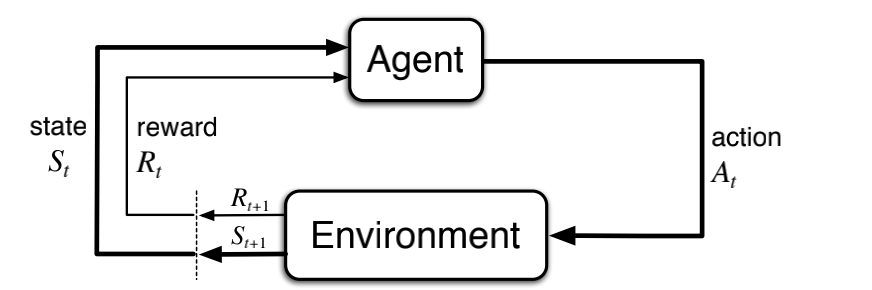
\includegraphics[scale=0.6]{MDP.png}
    \end{center}
    $\pi^\prime$
    RL considers solving Markov Decision Process (MDP)\\
    A policy a \sim \pi(.|\theta)\\
    Sample a trajectory from \pi : s_t \rightarrow a_t \sim \pi(.|s_t) \rightarrow r_t \rightarrow st+1 \rightarrow ...\\
    the object :\\
    \begin{center}
        \pi ^ * = \underset{\pi}{\argmax}J^\gamma(\pi)  = \underset{\pi}{\argmax} \EX(\overset{N-1}{\underset{n=1}{\sum}} r_n\gamma^n)\\
    \end{center}
\end{frame}

\begin{frame}
\frametitle{Value Based Method}
Many methods in reinforcement learning approach rely on learning a value function like Q-value to find the optimal policy. Where 
\begin{center}
    $Q(s_t,a_t) = \mathbb{E}[r(s_t,a_t) + \gamma Q(s_{t+1},a_{t+1})]$
\end{center}
Q-learning:
\begin{center}
    $Q(s_t,a_t) = Q(s_t,a_t) + \alpha [R_{t+1} + \gamma max_a Q(s_{t+1},a) - Q(s_t,a_t)]$
\end{center}
Once we have Q-value, an optimal policy can be easily found
\begin{center}
    $\pi(s) = argmax_a Q(s,a)$
\end{center}
This approach is Value-Based Method.

\end{frame}

\subsection{Policy Gradient}
\begin{frame}{Policy Gradient}
Another approach is Policy-Based Method. Instead of learn a value function, this approach directly learn a approximate policy function with paremeter $\theta$ based on gradient of object function.
\begin{center}
\theta_{t+1}
$&= \theta_t + \alpha \nabla_\theta \mathcal{J}(\pi_{\theta_t})$
\end{center}
where $\nabla \mathcal{J}(\pi_\theta)$ can be computed by using \textit{policy gradient theorem}:

\begin{center}
$\nabla_{\theta} \mathcal{J}_{\pi_\theta}
&= \mathbb{E}_{\pi_\theta}[V^{\pi_\theta}(s_0)]\\
&= \mathbb{E}_{\pi_\theta}[\nabla_{\theta} \text{log}  {\pi_\theta}(a|s)      Q^{\pi_\theta}(s,a)]$
\end{center}
    
\end{frame}


%---------------------------------------------------------

\section{DDPG}

\begin{frame}{DDPG - Main Idea}
The main idea of DDPG is combining DPG and DQN. \\
\vspace{0.2cm}
     
DQN is an algorithm built to solve large-dimensional tasks in state space by combining basic Q-learning algorithm and neural network.
\\
\begin{center}
     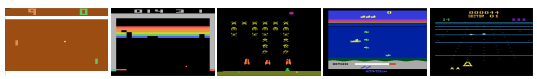
\includegraphics[scale=0.5]{Atarigame.png}
\end{center}
Specifically, DQN learns an approximation of the function Q based on the basic Q-learning algorithm.
 \begin{center}
        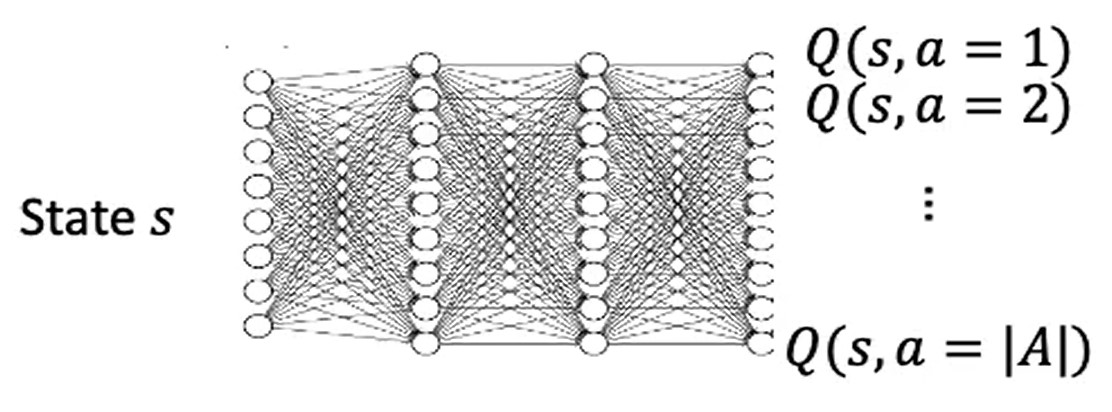
\includegraphics[scale=0.25]{net.jpg}
    \end{center}
With the policy being a greedy policy 
\begin{center}
    $\pi(s) = argmax_a Q(s,a)$
\end{center}
\end{frame}
\begin{frame}{DDPG - Main Idea}
DQN \textbf{only} works in an environment with a discrete action space. This is because in a task with a continuous action space, it is not possible to find Q-value for all actions and apply a greedy policy to choose the action that has a maximum Q-value
\begin{center}
    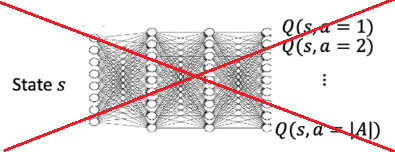
\includegraphics[scale=0.7]{Qoncontinuous.png}
\end{center}
\vspace{0.5cm}

\pause To solve this problem, DDPG algorithm uses an actor-critic architecture based on the DPG algorithm.
And to extend the DPG algorithm to solve continuous control tasks, DPG uses a neural network as an approximation function like the DQN algorithm. 
\end{frame}



\begin{frame}{DDPG - Main Idead}
The DPG algorithm maintains :
\begin{itemize}
    \item Actor $\mu(s|\theta^\mu)$ with a parameter
$\theta^\mu$ representing a deterministic policy of the agent, which
deterministic mapping a state to a specific action.
Update using deterministic policy gradient theorem
\begin{center}
$\nabla_{\theta^\mu}J
\approx \mathbb{E}_{s_t \sim p^\beta}[\nabla_{\theta^\mu} Q(s,a|\theta^Q)|_{s=s_t,a=\mu(s_t|\theta^\mu)}]$\\
\vspace{0.15cm}
$=  \mathbb{E}_{s_t \sim p^\beta}[\nabla_a Q(s,a|\theta^Q)|_{s=s_t,a=\mu(s_t)}\nabla_{\theta^\mu}\mu(s|\theta_\mu)|_{s_t}]$
\end{center}\\
\vspace{0.5cm}\pause
    \item Critic $Q(s,a|\theta^Q)$ with a parameter $\theta^Q$ use
    to learn Q function, showing how well the action is
chosen by the actor. Update by minimizing loss:
\begin{center}
$L = \mathbb{E}[(y_t - Q(s_t,a_t|\theta_Q))^2] $
\end{center}\\
where 
\begin{center}
$y_t = r(s_t,a_t) + \gammaQ(s_{t+1},\mu(s_{t+1}|\theta^Q)$
\end{center}
\end{itemize} 
\end{frame}

\begin{frame}{DDPG-Replay buffer and Target Network}
DDPG algorithm borrows the idea of using \textit{replay buffer} and \textit{target networks} from DQN algorithm.\\
\vspace{0.5cm}
\pause 
Replay buffer use to store experience when the agent interacts with the environment, this makes for better learning because when randomly taking experience from the replay buffer to break the correlation between consecutive samples.\\
\pause
\vspace{0.5cm}
Target networks use to keep learning stable by frozen the target value. Update by using \textit{soft update}: $\theta' = \tau\theta + (1-\tau)\theta'$ with $\tau \ll 1$.\pause Changing to soft-update causes the target network to change slowly, greatly improving the stability of learning. 
\end{frame}

\begin{frame}{Exploration}
One problem with deterministic policies is that it often quickly converges to produce the same actions while not exploring enough, thereby ignoring states that might lead to a higher total expected reward. To address this problem, the DDPG algorithm constructs an exploration policy $\mu'$ by adding noise to the actor policy
\begin{center}
$\mu'(s_t) = \mu(s_t) + \mathcal{N}$
\end{center}
$\mathcal{N}$ can be anything, DDPG's author choice is to use Ornstein-Uhlenbeck process.
\end{frame}


\begin{frame}{DDPG - Pseudocode}
\begin{center}
     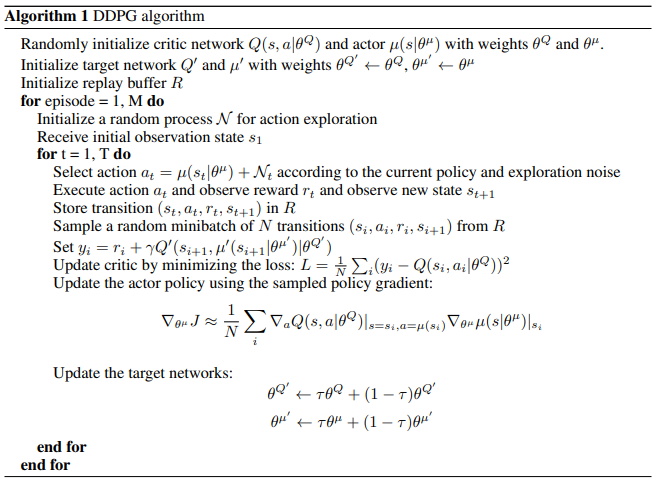
\includegraphics[scale=0.63]{DDPG-Pseudocode.png}
\end{center}
   
\end{frame}

    

%---------------------------------------------------------

\section{SAC}

\subsection{Entropy}

\begin{frame}{Entropy}
In RL, entropy refers to the predictability of the actions of an agent.\\
This is closely related to the certainty of its policy about what action will yield the highest cumulative reward in the long run: if certainty is high, entropy is low and vice versa
    \begin{center}
        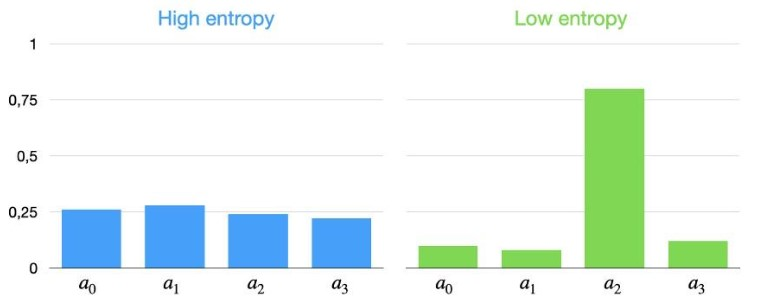
\includegraphics[scale=0.6]{entropy.jpg}\\
    \end{center}
\end{frame}

\begin{frame}{Entropy}
    With x is a random variable with probability mass function P(X)\\
    Etropy can be calculated by
    \begin{center}
        $H(X) = - \underset{x \in X}{\sum} P(x)logP(x)$\\
    \end{center}
    In RL we want to calcutate the entropy of policy \pi\\
    The equation now become\\
    \begin{center}
        $H(\pi(.|s_t)) = - \underset{a \in A}{\sum} \pi(a|s_t)log\pi(a|s_t)$\\
    \end{center}
    To do that we need the policy \pi is a Probability distribution \\
    So that the SAC actor need to be a Stochastic Actor
\end{frame}

\subsection{Stochastic Actor}

\begin{frame}{Stochastic Actor}
    Unlike DDPG and TD3 what give directly  the action vector given a state vector\\
    A Stochastic Actor will give mean and covariance \\
    Then use the Gaussian distribution with mean and coveriance to make a action vector\\
\end{frame}

\subsection{soft actor-critic}

\begin{frame}{soft actor-critic}
    SAC is an off-policy algorithm that is built on the actor-critic framework.\\
    The algorithm push a entropy of policy in RL objective function. The RL objective function now become\\
    \begin{center}
        $J(\pi) =\overset{T}{\underset{t=0}{\sum}}\underset{(s_t,a_t) \sim \pi}{\EX}[r(s_t,a_t) + \alpha H(\pi(.|s_t))]$\\ 
    \end{center}
    The policy now need to learn how to maximize the reward and the entropy at the same time\\
\end{frame}

\begin{frame}{soft actor-critic Pseudocode}
    \begin{algorithm}[H]
        \KwData{\lambda_\psi, \lambda_{\theta_1}, \lambda_{\theta_2}, \lambda_\phi, \tau}
        Initialize parameter vectors \psi,\hat{\psi}, \theta_1.\theta_2,\phi \\
        \For{each iteration}{
            \For{each step in environment}{
                a_t \sim \pi_\phi(a_t,s_t)\\
                s_{t+1} \sim p(s_{t+1}|s_t,a_t)\\
                D \leftarrow D \cup (s_t,a_t,r,s_{t+1})\\
            }
            \EndFor\\
            \For{each gradient step}{
                \psi \leftarrow \psi - \lambda_\psi \nabla_\psi J_V(\psi)\\
                \For{i in {1,2}}{
                    \theta_i \leftarrow \theta_i - \lambda_\theta_i \nabla_\theta_i J_Q(\theta_i) \\
                }
                \EndFor
                \phi \leftarrow \phi - \lambda_\phi \nabla_\phi J_\pi(\phi)\\
                \psi \leftarrow \tau\psi + (1-\tau)\hat{\psi}\\
            }
            \EndFor
        }
        \EndFor
    \end{algorithm}
\end{frame}
\begin{frame}{soft actor-critic }
    We will consider some neural network to describe:\\
    state value function: V_\psi(s_t)\\
    soft Q function: Q_\theta(s_t,a_t)\\
    policy: \pi_\phi(a_t|s_t)\\
    The parameters of these network are \psi,\theta,\phi.\\
    
\end{frame}

\begin{frame}{soft actor-critic }
    The soft value function is trained to minimize the squared residual error\\
    \begin{center}
        $J_v(\psi) = \EX_{s_t \sim D}[1/2(V_\psi(s_t) - \EX_{a_t \sim \pi_\phi}[Q_\theta(s_t,a_t) - log\pi_\phi(a_t|s_t)])^2]$\\
    \end{center}
    The gradient it can be estimated by\\
    \begin{center}
        $\nabla_\psi J_V(\psi) = \nabla_\psi V_\psi(s_t)(V_\psi(s_t) - Q_\theta(s_t,a_t) + log\pi_\phi(a_t,s_t))$\\
    \end{center}
\end{frame}

\begin{frame}{soft actor-critic}
    The soft Q-function parameters can be trained to minimize the soft Bellman residual\\
    \begin{center}
        $J_Q(\theta) = \EX_{(s_t,a_t) \sim D} [1/2(Q_\theta(s_t,a_t) - \hat{Q}(s_t,s_t))^2]$\\
    \end{center}
    with\\
    \begin{center}
        $\hat{Q}(s_t,s_t) = r(s_t,s_t) + \gamma\EX_{s_t+1 \sim p}[ {V_\hat{\psi}(s_t,a_t)} ]$\\
    \end{center}
    can be optimized with stochastic gradients\\
    \begin{center}
        $\nabla_\theta J_Q(\theta) = \nabla_\theta Q_\theta(s_t,a_t) - r(s_t,a_t) - {\gamma V_\hat{\psi}(s_{t+1})})$\\
    \end{center}
\end{frame}

\begin{frame}{soft actor-critic}
    Finally, the policy parameters can be learned by directly minimizing the objective function\\
    \begin{center}
        $J_\pi(\phi) = \EX_{s_t \sim D, \epsilon \sim N} [log \pi_\phi(f_\phi(\epsilon,s_t)|s_t) - Q_\phi (s_t,f_\phi(\epsilon_t;s_t))]$\\
    \end{center}
    We can approximate the gradient with\\
    \begin{center}
        $\nable_\phi J_\pi(\phi) = \nabla_\phi log\pi_\phi(a_t,s_t) \\
        + (\nabla_{a_t}log\pi_\phi(a_t,s_t) - \nabla_{a_t}Q(s_t,a_t)) \nabla_\phi f_\phi(\epsilon;s_t) $ \\
        
    \end{center}
\end{frame}

%---------------------------------------------------------

\section{TD3}
\begin{frame}{TD3 - Overestimation Bias}
    \begin{itemize}
\onslide<1->{
        \item TD3 addresses overestimation bias.
        }
\onslide<2-> {
        \vspace{0.5cm}
        \item Overestimation bias occurs when estimated values $Q_{θ}(s, a)$ \\
        are in general greater than true values $Q(s, a)$.
        %, thus the agent overestimates the expected future rewards. Policy seeks these erroneous overestimations and exploits them. It may lead to poor policy performance and propagation of estimation errors.
        }
\onslide<3-> {
        \vspace{0.5cm}
        \item In Q-Learning we get bias from the max over actions.
        $$y=r+\gamma \max _{a^{\prime}} Q\left(s^{\prime}, a^{\prime}\right)$$
        % Also in DDPG. General, in Actor-Critic?
        }
        \end{itemize}
\end{frame}


\begin{frame}{TD3 - Overestimation Bias}
    \begin{itemize}
\onslide<1->{
        \item Overestimation also comes from approximation errors.
        % All approximation. Neural Network too.
        }
\onslide<2-> {
        \vspace{0.5cm}
        \item AC methods are bootstrapped so errors accummulate.
        \begin{equation*}
        \begin{split}
            &Q_{\theta}\left(s_{t}, a_{t}\right)=r_{t}+\gamma \mathbb{E}\left[Q_{\theta}\left(s_{t+1}, a_{t+1}\right)\right]-\delta_{t} \\
            &=r_{t}+\gamma \mathbb{E}\left[r_{t+1}+\gamma \mathbb{E}\left[Q_{\theta}\left(s_{t+2}, a_{t+2}\right)-\delta_{t+1}\right]\right]-\delta_{t} \\
            &=\mathbb{E}_{s_{i} \sim p_{\pi}, a_{i} \sim \pi}\left[\sum_{i=t}^{T} \gamma^{i-t}\left(r_{i}-\delta_{i}\right)\right]
        \end{split}
        \end{equation*}
        }
\onslide<3-> {
        \item TD3's solution:
        $$y \leftarrow r+\gamma \min _{i=1,2} Q_{\theta_{i}^{\prime}}\left(s^{\prime}, 
        \pi_{\theta_1}(s^{\prime})\right)$$
        }
        \end{itemize}
\end{frame}


\begin{frame}{TD3 - Pseudocode}
\only<1>{
    Initialize critic networks $Q_{\theta_{1}}, Q_{\theta_{2}}$, and actor network $\pi_{\phi}$ \\
    with random parameters $\theta_{1}, \theta_{2}, \phi$ \\
    Initialize target networks $\theta_{1}^{\prime} \leftarrow \theta_{1}, \theta_{2}^{\prime} \leftarrow \theta_{2}, \phi^{\prime} \leftarrow \phi$ \\
    Initialize replay buffer $\mathcal{B}$ \\
    for $t=1$ to $T$ do \\
        \quad Select action with exploration noise $a \sim \pi_{\phi}(s)+\epsilon$, \\
        \quad ${\epsilon \sim \mathcal{N}(0, \sigma)}$ and observe reward $r$ and new state $s^{\prime}$ \\
        \quad Store transition tuple $\left(s, a, r, s^{\prime}\right)$ in $\mathcal{B}$ \\
        }
\only<2>{
    \quad Sample mini-batch of $N$ transitions $\left(s, a, r, s^{\prime}\right)$ from $\mathcal{B}$ \\
    \quad $\tilde{a} \leftarrow \pi_{\phi^{\prime}}\left(s^{\prime}\right)+\epsilon, \quad {\epsilon \sim \operatorname{clip}(\mathcal{N}(0, \tilde{\sigma}),-c, c)}$ \\
    \quad $y \leftarrow r+\gamma \min _{i=1,2} Q_{\theta_{i}^{\prime}}\left(s^{\prime}, \tilde{a}\right)$ \\
    \quad Update critics $\theta_{i} \leftarrow \operatorname{argmin}_{\theta_{i}} N^{-1} \sum\left(y-Q_{\theta_{i}}(s, a)\right)^{2}$ \\
    \quad if $t$ mod $d$ then \\
        \quad \quad Update $\phi$ by the deterministic policy gradient: \\
        \quad \quad ${\nabla_{\phi} J(\phi)=\left.N^{-1} \sum \nabla_{a} Q_{\theta_{1}}(s, a)\right|_{a=\pi_{\phi}(s)} \nabla_{\phi} \pi_{\phi}(s)}$ \\
        \quad \quad Update target networks: \\
        \quad \quad ${\theta_{i}^{\prime} \leftarrow \tau \theta_{i}+(1-\tau) \theta_{i}^{\prime}}$ \\
        \quad \quad ${\phi^{\prime} \leftarrow \tau \phi+(1-\tau) \phi^{\prime}}$ \\
    \quad end if \\
    end for
}

\end{frame}




%---------------------------------------------------------

\section{Comparison}

\begin{frame}{Comparison}
\begin{center}
\only<1> {
    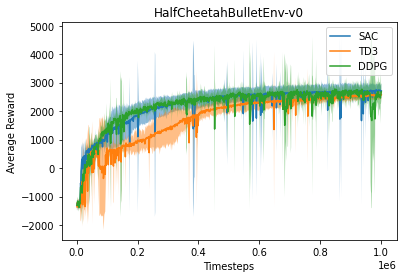
\includegraphics[scale=0.7]{halfcheetah.png}
}
\only<2> {
    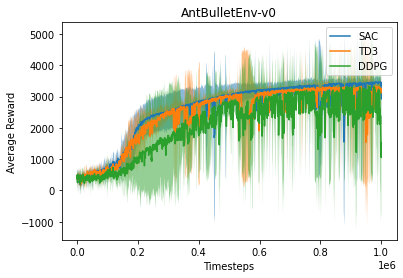
\includegraphics[scale=0.7]{antbullet.png}
}
\only<3> {
    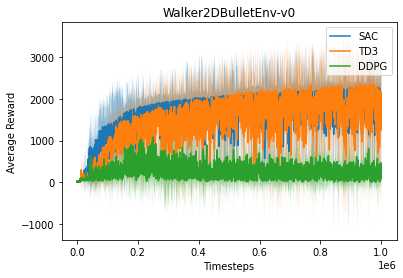
\includegraphics[scale=0.7]{walker.png}
}
\end{center}
\end{frame}

\begin{frame}
\begin{center}
    
\includegraphics[scale=0.5]{thank.jpg}
\end{center}
\end{frame}

\end{document}